\documentclass[11pt]{article}
\usepackage[margin=0.82in]{geometry}
\usepackage{booktabs}
\usepackage{array}
\usepackage{xcolor}
\usepackage{pgfplots}
\usepackage{graphicx}
\usepackage{amsmath}
\usepackage{hyperref}
\usepackage{enumitem}
\usepackage{parskip}

\pgfplotsset{compat=1.18}
\definecolor{siamese}{HTML}{2A6F97}
\definecolor{classical}{HTML}{2F8F6B}

\hypersetup{
  colorlinks=true,
  linkcolor=black,
  urlcolor=siamese
}
\emergencystretch=3em

\title{\textbf{Substrate-Agnostic SERS Classification}\\
\large Quick supervisor summary}
\author{}
\date{\today}

\begin{document}
\maketitle

\section*{Summary}

The earlier SERS Siamese work was effectively a \textbf{chemical-substrate pair classifier}. The model learned classes such as \texttt{4np\_\_AgNP}, \texttt{pyridine\_\_PICO}, and \texttt{bt\_\_pSERS}. That is useful for distinguishing measured pair conditions, but it does not establish substrate-agnostic detection.

The current work changes the task. The model now predicts \textbf{chemical identity only} and is evaluated by holding out an entire substrate family during training. This is the relevant test: if a substrate family is absent during training, can the model still identify the chemical on that held-out family?

\begin{center}
\begin{tabular}{p{0.38\linewidth}rrrr}
\toprule
\textbf{Method} & \textbf{Accuracy} & \textbf{Bal. acc.} & \textbf{Macro F1} & \textbf{Weakest fold} \\
\midrule
Previous chemical-substrate Siamese evaluation & 0.854 & 0.854 & 0.686 & 0.380 \\
Best substrate-agnostic Siamese & 0.975 & 0.975 & 0.977 & \texttt{Ag}: 0.920 \\
K-shot Siamese check, $K=5$ & 0.873 & 0.873 & 0.850 & \texttt{pSERS}: 0.333 \\
Best classical baseline & 0.987 & 0.987 & 0.987 & \texttt{Ag}: 0.960 \\
Raw-spectrum Siamese control & 0.440 & 0.440 & 0.399 & \texttt{Au}: 0.000 \\
\bottomrule
\end{tabular}
\end{center}

\begin{figure}[ht]
\centering
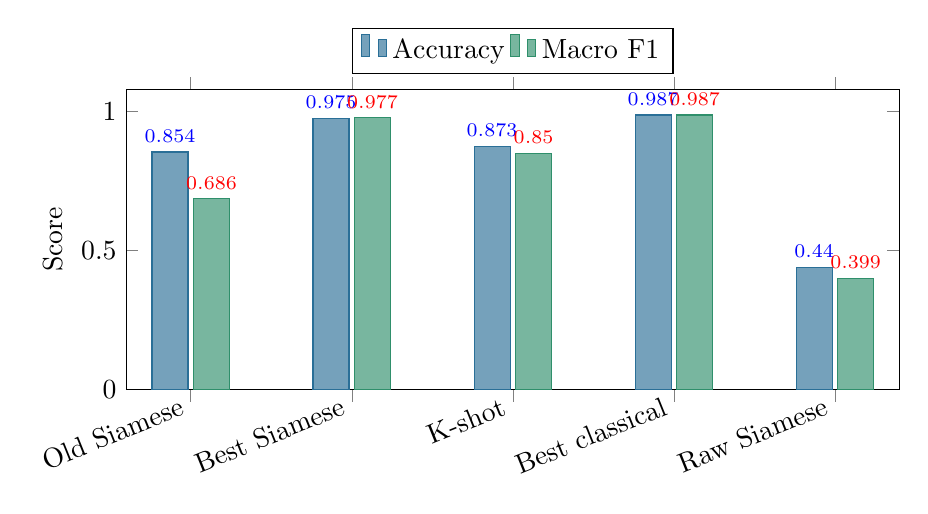
\begin{tikzpicture}
\begin{axis}[
  ybar,
  width=0.94\linewidth,
  height=5.4cm,
  ymin=0,
  ymax=1.08,
  ylabel={Score},
  symbolic x coords={Old Siamese,Best Siamese,K-shot,Best classical,Raw Siamese},
  xtick=data,
  x tick label style={rotate=22,anchor=east},
  bar width=13pt,
  legend style={at={(0.5,1.05)},anchor=south,legend columns=2},
  nodes near coords,
  nodes near coords style={font=\scriptsize,/pgf/number format/fixed,/pgf/number format/precision=3},
]
\addplot+[fill=siamese!65,draw=siamese] coordinates {
  (Old Siamese,0.854) (Best Siamese,0.975) (K-shot,0.873) (Best classical,0.987) (Raw Siamese,0.440)
};
\addplot+[fill=classical!65,draw=classical] coordinates {
  (Old Siamese,0.686) (Best Siamese,0.977) (K-shot,0.850) (Best classical,0.987) (Raw Siamese,0.399)
};
\legend{Accuracy,Macro F1}
\end{axis}
\end{tikzpicture}
\caption{Main result comparison. For the grouped runs, macro F1 is computed over the true labels present in each held-out fold. The K-shot result uses $K=5$ support spectra per held-in chemical-substrate-family cell. The best substrate-agnostic Siamese model performs well, but the best non-deep baseline is slightly better on this small dataset. Raw spectra perform poorly, confirming that derivative preprocessing is important.}
\end{figure}

\section*{Dataset And Evaluation}

The current substrate-agnostic evaluation uses 275 spectra from three chemicals: \texttt{4np}, \texttt{benzenethiol}, and \texttt{pyridine}. The current matrix is:

\begin{center}
\begin{tabular}{lrrrr}
\toprule
\textbf{Chemical} & \textbf{Ag} & \textbf{Au} & \textbf{PICO} & \textbf{pSERS} \\
\midrule
\texttt{4np} & 25 & 0 & 25 & 25 \\
\texttt{benzenethiol} & 25 & 25 & 25 & 25 \\
\texttt{pyridine} & 25 & 25 & 25 & 25 \\
\texttt{n,n-dimethylformamide} & 0 & 228 & 0 & 0 \\
\bottomrule
\end{tabular}
\end{center}

\begin{figure}[ht]
\centering
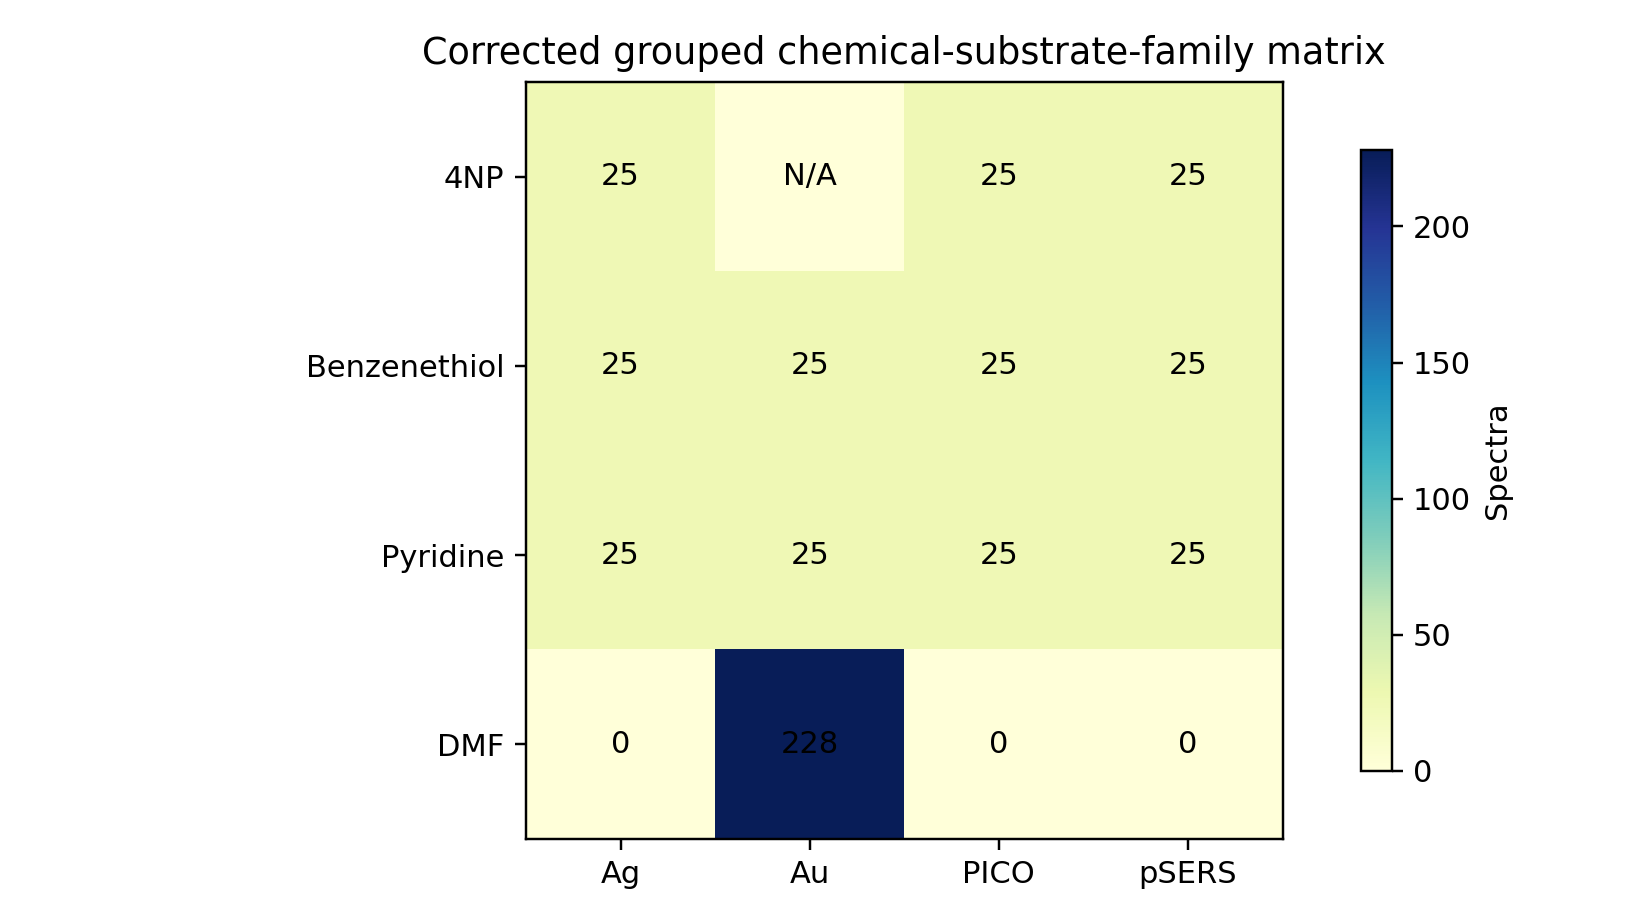
\includegraphics[width=0.68\linewidth]{figures/corrected_dataset_matrix.png}
\caption{Current chemical-substrate-family matrix. DMF is present but only on Au, so it is not part of the current substrate-agnostic model.}
\end{figure}

Testing is \textbf{leave-one-substrate-family-out}. Each fold removes one full substrate family from training and tests on that held-out family:

\begin{center}
\begin{tabular}{lrrp{0.42\linewidth}}
\toprule
\textbf{Held-out family} & \textbf{Train} & \textbf{Test} & \textbf{Test chemicals} \\
\midrule
\texttt{Ag} & 200 & 75 & \texttt{4np}, \texttt{benzenethiol}, \texttt{pyridine} \\
\texttt{Au} & 225 & 50 & \texttt{benzenethiol}, \texttt{pyridine} \\
\texttt{PICO} & 200 & 75 & \texttt{4np}, \texttt{benzenethiol}, \texttt{pyridine} \\
\texttt{pSERS} & 200 & 75 & \texttt{4np}, \texttt{benzenethiol}, \texttt{pyridine} \\
\bottomrule
\end{tabular}
\end{center}

This prevents direct memorization of the held-out substrate-family spectra. The remaining limitation is dataset size and independence: 25 spectra from one map are not equivalent to 25 independent preparations.

\section*{Preprocessing}

The report notes a low-wavenumber device artifact below approximately 300 cm$^{-1}$. The current pipeline keeps only 330.906 to 1797.919 cm$^{-1}$, giving 663 spectral input points.

The best Siamese model uses first-derivative spectra:

\begin{enumerate}[leftmargin=*]
\item crop the spectrum to 330--1800 cm$^{-1}$;
\item apply per-spectrum standard normal variate normalization;
\item apply a Savitzky-Golay first derivative with window length 17 and polynomial order 3;
\item L2-normalize the final vector.
\end{enumerate}

The best classical baseline uses the same idea but with the \textbf{second derivative}. The second derivative emphasizes peak curvature and suppresses broad baseline/background structure more strongly.

\section*{Best Siamese Model}

The best substrate-agnostic Siamese model keeps the original metric-learning idea but changes the label and evaluation. It learns a 64-dimensional chemical embedding and classifies by nearest chemical prototype.

\begin{center}
\begin{tabular}{p{0.30\linewidth}p{0.58\linewidth}}
\toprule
\textbf{Component} & \textbf{Current setting} \\
\midrule
Input & First-derivative, SNV-normalized, L2-normalized SERS spectrum. \\
Encoder & Conv1D 1$\rightarrow$16, ReLU, max pool; Conv1D 16$\rightarrow$32, ReLU, max pool; flatten; linear layer to 64 dimensions; ReLU; L2 embedding normalization. \\
Loss & Triplet loss with margin 0.2. \\
Triplet sampling & Anchor and positive share chemical identity; cross-substrate positives are preferred. Negative has a different chemical; same-substrate negatives are preferred when available. \\
Training & 100 epochs, batch size 32, Adam learning rate $10^{-3}$, small Gaussian noise and spectral-shift augmentation. Training is run on GPU. \\
Inference & Embed training spectra, compute row-mean chemical prototypes, classify held-out spectra by nearest prototype. \\
\bottomrule
\end{tabular}
\end{center}

Fold-level performance:

\begin{center}
\begin{tabular}{lrrrp{0.32\linewidth}}
\toprule
\textbf{Held-out} & \textbf{Accuracy} & \textbf{Bal. acc.} & \textbf{Macro F1} & \textbf{Main error} \\
\midrule
\texttt{Ag} & 0.920 & 0.920 & 0.919 & 6/25 \texttt{4np} predicted as \texttt{benzenethiol}. \\
\texttt{Au} & 0.980 & 0.980 & 0.990 & 1/25 \texttt{benzenethiol} predicted as \texttt{4np}. \\
\texttt{PICO} & 1.000 & 1.000 & 1.000 & None. \\
\texttt{pSERS} & 1.000 & 1.000 & 1.000 & None. \\
\bottomrule
\end{tabular}
\end{center}

The saved CSV reports \texttt{0.660} macro F1 for the held-out \texttt{Au} fold because \texttt{4np} is not a true Au test class, but one spectrum is falsely predicted as \texttt{4np}. That default macro average includes the absent class and is not a fair fold-level summary. The table above reports macro F1 over the true labels present in each fold.

\begin{figure}[ht]
\centering
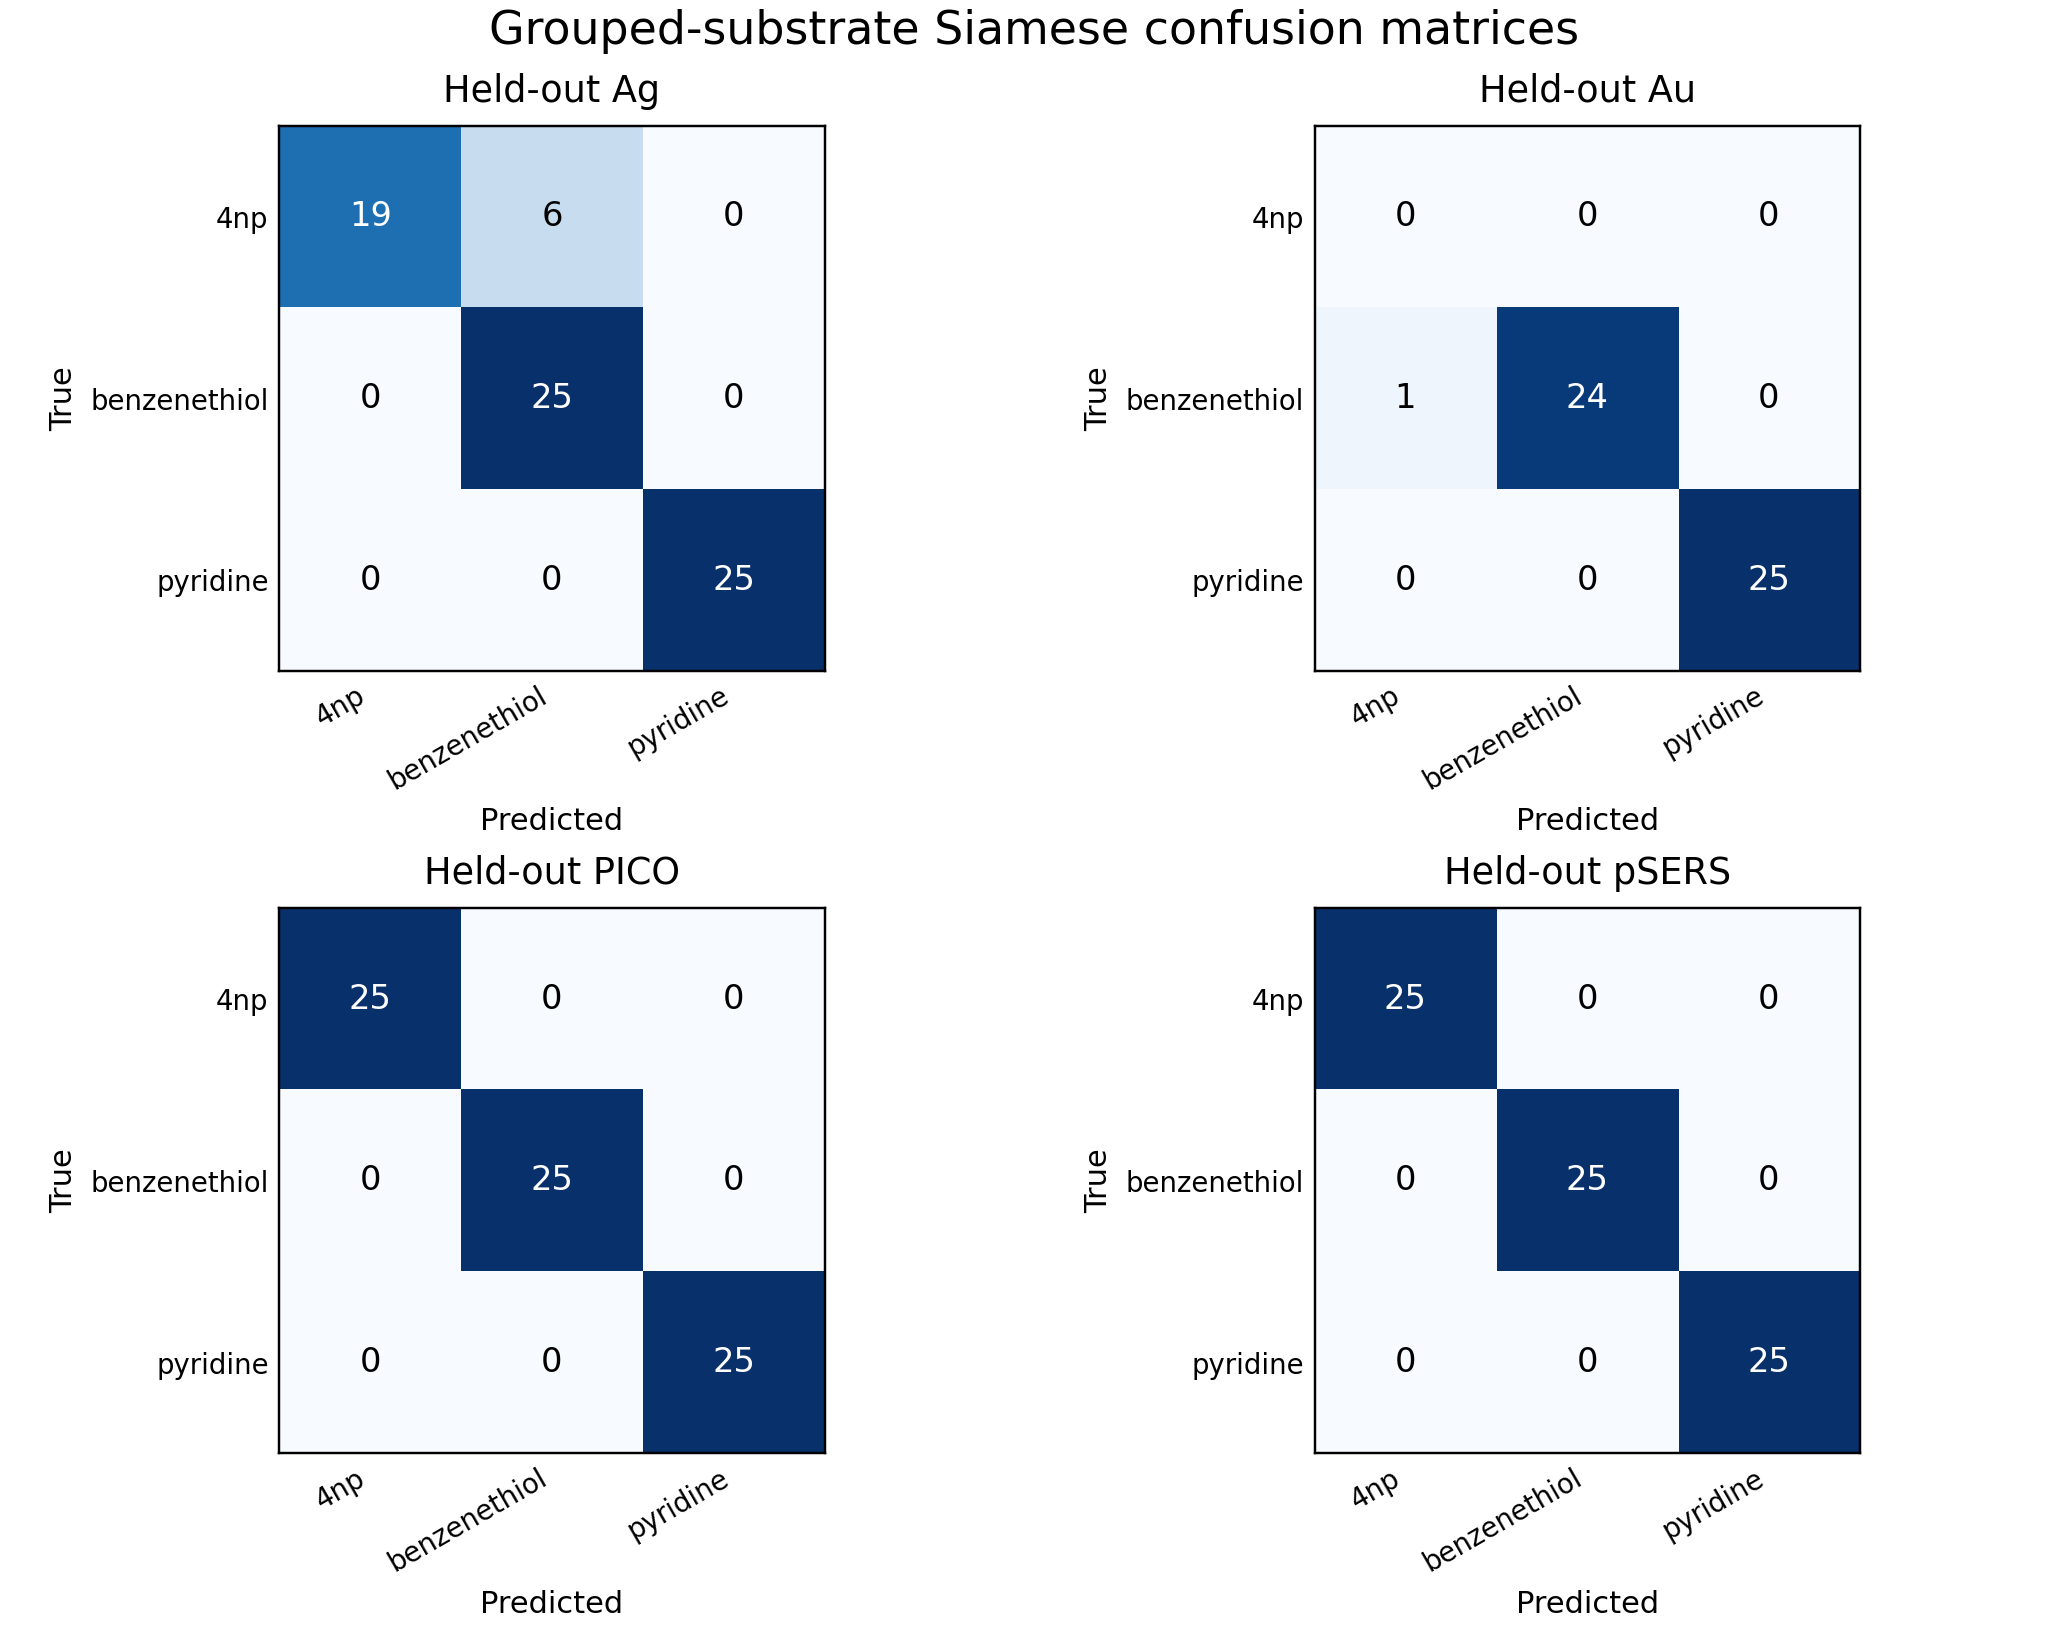
\includegraphics[width=0.86\linewidth]{figures/grouped_best_confusions.png}
\caption{Best Siamese confusion matrices. The only meaningful failure mode is \texttt{4np} in the held-out Ag fold being pulled toward \texttt{benzenethiol}.}
\end{figure}

\section*{Formal K-Shot Check}

The submitted abstract used the phrase few-shot because the original chemical-substrate pair model was trained from a small number of spectra per measured pair. I tested whether that claim still holds in the harder substrate-agnostic setting by restricting training to $K$ support spectra per held-in chemical-substrate-family cell, while keeping the same leave-one-substrate-family-out test. The encoder, triplet loss, prototype inference, first-derivative preprocessing, and GPU-only training setup were unchanged.

\begin{center}
\begin{tabular}{rrrr}
\toprule
\textbf{K} & \textbf{Mean acc.} & \textbf{Mean true-label macro F1} & \textbf{Worst fold acc.} \\
\midrule
1 & 0.913 & 0.905 & 0.653 \\
3 & 0.840 & 0.819 & 0.000 \\
5 & 0.873 & 0.850 & 0.333 \\
10 & 0.874 & 0.853 & 0.560 \\
25 & 0.930 & 0.924 & 0.600 \\
\bottomrule
\end{tabular}
\end{center}

This is useful evidence, but it is not strong enough to claim a robust few-shot substrate-agnostic detector. The K-shot runs are high variance because support selection and triplet training matter at this dataset size. A precise wording is: \textbf{Siamese metric learning for substrate-agnostic SERS classification on a small dataset, with a formal K-shot stress test.}

\section*{Best Classical Baseline}

The best non-deep-learning baseline is:

\begin{center}
\textbf{second derivative + nearest centroid}
\end{center}

This model computes the second-derivative feature vector for every spectrum. During each leave-one-substrate-family-out fold, it computes the centroid of each chemical class from the training substrate families. A held-out test spectrum is assigned to the chemical whose centroid is closest in Euclidean distance.

\begin{center}
\begin{tabular}{llrrr}
\toprule
\textbf{Feature} & \textbf{Model} & \textbf{Accuracy} & \textbf{Bal. acc.} & \textbf{Macro F1} \\
\midrule
\texttt{derivative\_2} & nearest centroid & 0.987 & 0.987 & 0.987 \\
\texttt{derivative\_1} & nearest centroid & 0.973 & 0.973 & 0.973 \\
\texttt{peak\_emphasis} & nearest centroid & 0.963 & 0.963 & 0.963 \\
\texttt{derivative\_2} & cosine kNN, $k=3$ & 0.950 & 0.950 & 0.946 \\
\bottomrule
\end{tabular}
\end{center}

This baseline is important because it is simpler than the Siamese model and slightly stronger on the current dataset. The spectra are already well organized in derivative space for these three chemicals. Future deep models should be compared against this baseline, not only against the old Siamese pair-classification results.

\section*{Geometry Evidence}

The Siamese embedding improves chemical organization. Silhouette scores compare how close each spectrum is to its own group versus the nearest other group.

\begin{center}
\begin{tabular}{lrrr}
\toprule
\textbf{Space} & \textbf{Chemical silhouette} & \textbf{Substrate silhouette} & \textbf{Difference} \\
\midrule
Derivative input & 0.304 & 0.101 & 0.203 \\
K-shot Siamese embedding, $K=5$ & 0.748 & -0.042 & 0.789 \\
Siamese embedding & 0.797 & -0.040 & 0.837 \\
\bottomrule
\end{tabular}
\end{center}

The embedding therefore clusters spectra much more by chemical identity and less by substrate family. The $K=5$ embedding shows the same direction of improvement, but the full-data embedding is more stable and slightly more chemically organized.

\begin{figure}[ht]
\centering

\includegraphics[width=0.82\linewidth]{figures/silhouette_scores_by_fold.png}
\caption{Chemical-label and substrate-family silhouette scores by held-out fold.}
\end{figure}

\begin{figure}[ht]
\centering
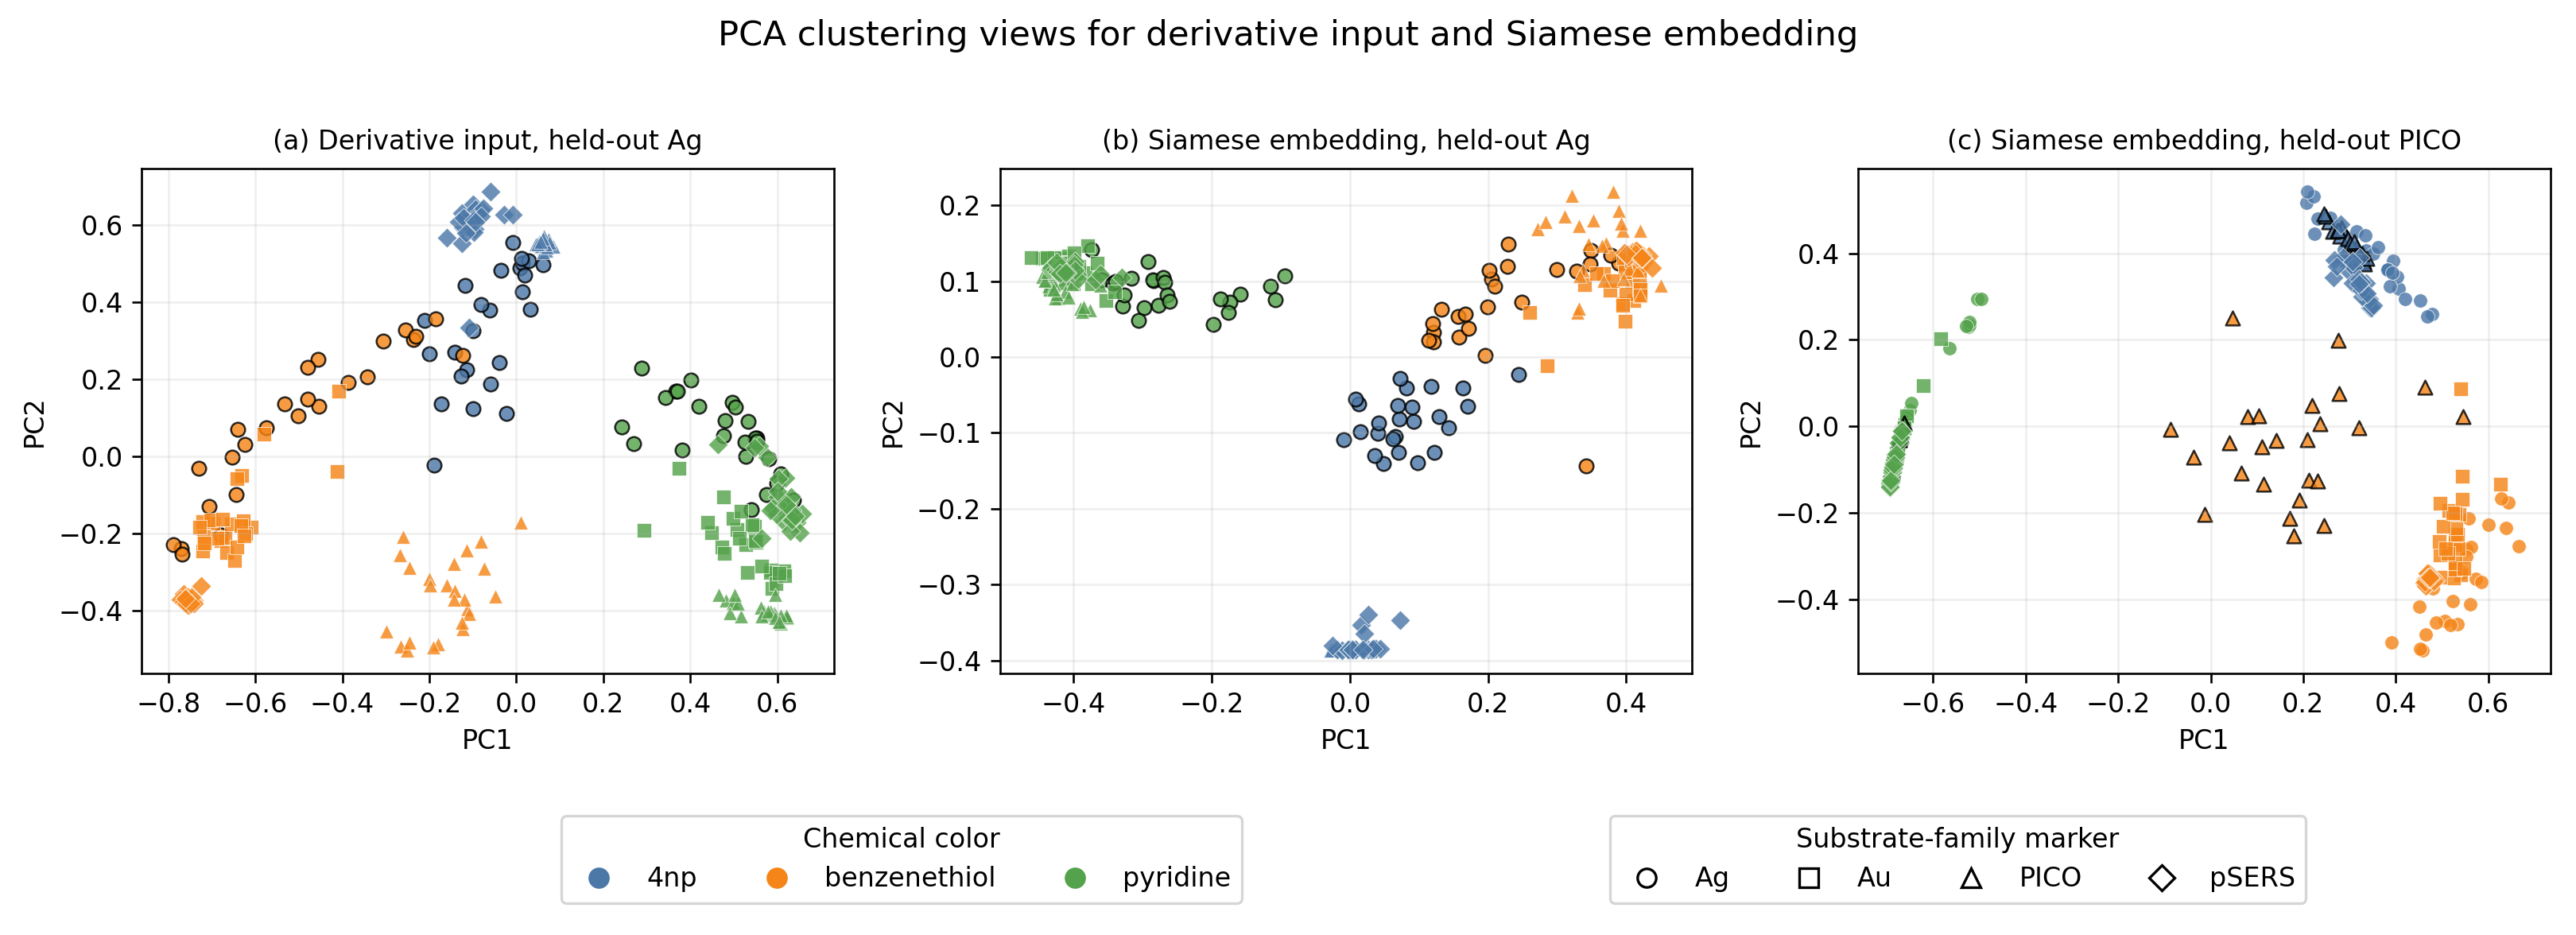
\includegraphics[width=\linewidth]{figures/combined_pca_clustering.png}
\caption{PCA clustering views. (a) Derivative-input PCA for held-out Ag. (b) Siamese-embedding PCA for held-out Ag. (c) Siamese-embedding PCA for held-out PICO. Color indicates chemical identity; marker shape indicates substrate family.}
\end{figure}

\section*{Interpretation And Next Steps}

The current substrate-agnostic result is credible for the available three-chemical dataset, but it is not yet a broad SERS substrate-agnostic detector. The evidence is strongest for \texttt{benzenethiol} and \texttt{pyridine}, which are measured on all four substrate families. \texttt{4np} is valid on three substrate families but remains the main weak class in the held-out Ag fold. The formal K-shot check supports the same direction of progress, but its fold variance shows that the current dataset is still too small for a strong few-shot substrate-agnostic claim.

The next dataset improvement should be to add another responsive chemical across all four substrate families. DMF is a candidate only if it responds reliably beyond Au.

The phrase ``25 spectra per chemical-substrate-family cell'' should be treated only as a short-term \textbf{minimum matrix-fill target}. It is enough to make a new cell usable in leave-one-substrate-family testing, but it is not a sufficient dataset size for robust deep learning. Siamese models help in small-data settings because they generate many pairs or triplets from limited spectra, but those pairs do not create new independent chemical or substrate variation.

For a stronger substrate-agnostic deep-learning claim, each new chemical-substrate-family cell should ideally include multiple independent preparations or maps, and preferably spectra collected across different sessions or days. More independent preparations are more valuable than simply collecting many correlated points from one map.

\section*{Bottom Line}

We have moved from chemical-substrate pair classification to a true chemical-label, leave-one-substrate-family-out evaluation. The best Siamese model reaches 0.975 mean accuracy, the formal $K=5$ check reaches 0.873 mean accuracy, and the best classical derivative baseline reaches 0.987. The current data support a strong proof of concept, but the next step for a stronger substrate-agnostic claim is another complete chemical across all substrate families plus more independent maps or preparations.

\end{document}
